%\chapter{Obsah CD}
\chapter{Inštalácia}
{
	V tejto kapitole by som Vád objasnil postup inštalácie aplikácie. V prvom rade uviediem potrebné prostriedky pre beh aplikácie. Pre správny beh aplikácie potrebujeme nasledovné prostriedky:
	\begin{itemize}
	\item JBoss aplikačný server najmenej vo verzii 7.1.1.Final. Je možné ho zdarma stiahnuť z http://jbossas.jboss.org/downloads
	\item MySQL Connector/J minimálne vo verzii 5.0.8, ktorý je súčasťou CD
	\item MySQL databázový server najmenej vo verzii 5.5.37(na distribúcií ubuntu je možné nainštalovať príkazom \uv{apt-get install mysql-server mysql-client}, alebo je možné postupovať podľa nasledujúceho návodu  \\http://dev.mysql.com/doc/refman/5.1/en/linux-installation.html)
	\item Webový prehlidač Mozilla Firefox najmenej vo verzii 29.0 alebo Google Chrome najmenej vo verzii 34.0(v prostredí ubuntu je možné ho nainštalovať nasledujúcim príkazom \uv{apt get install firefox/google-chrome})
	\end{itemize}
	V prvom rade je potrebné nainštalovať MySQL server nakonfigurovať databázu s názvom \uv{optaplanner} s užívateľským menom \uv{root} a heslom \uv{root}. Následne je potrebné rozbaliť stiahnutý JBoss aplikačný server na súborový systém. V ďalšom kroku nastaví náš aplikačný server pre správne použitie MySQL databáze.  To urobíme zkopírovaním súboru standalone-full.xml do adresára JBOSS\_HOME\footnote{JBOSS\_HOME predstavuje koreňový adresár serveru JBoss na disku}/standalone/configuration a prepíše aktuálny obsah súboru.

	Následne treba ovládač mysql-connector-java-5.1.29-bin.jar umiestniť do adresára \\ JBOSS\_HOME/standalone/deployments. Následne treba vytvoriť potrebnú databázu to a naplniť ju dátami :
	\begin{itemize}
	\item zadaním príkazu mysql -u root -p optaplanner < cesta/k/suboru/create.sql(bude od nás vyžadované heslo root, ktoré zadáme)
	\item zadaním príkazu mysql -u root -p optaplanner < cesta/k/suboru/insert.sql(bude od nás vyžadované heslo root, ktoré zadáme)
	\end{itemize}

	Nakoniec skopríruje súbor standalone.conf do adresára JBOSS\_HOME/bin a prepíše aktuálny obsah súboru.

	Aplikáciu môžme spustiť nasledovne:
	\begin{itemize}
	\item Skopírujeme adresára optaplanner.controlle.war do adresára \\ JBOSS\_HOME/standalone/deployments
	\item Skopírujeme súbor PlannerService.war do adresára \\ JBOSS\_HOME/standalone/deployments
	\item Prejdeme do zložky JBOSS\_HOME/standalone/bin a spustíme skript \emph{standalone.sh}
	\end{itemize}
	
	K aplikácií pristúpime zadaním adresy \uv{http://localhost:8080/optaplanner.controller.war/} do webového podporovaného webového prehliadaču.


}

\chapter{Užívatelské rozhranie}
{

\begin{figure}[htb]

\begin{center}

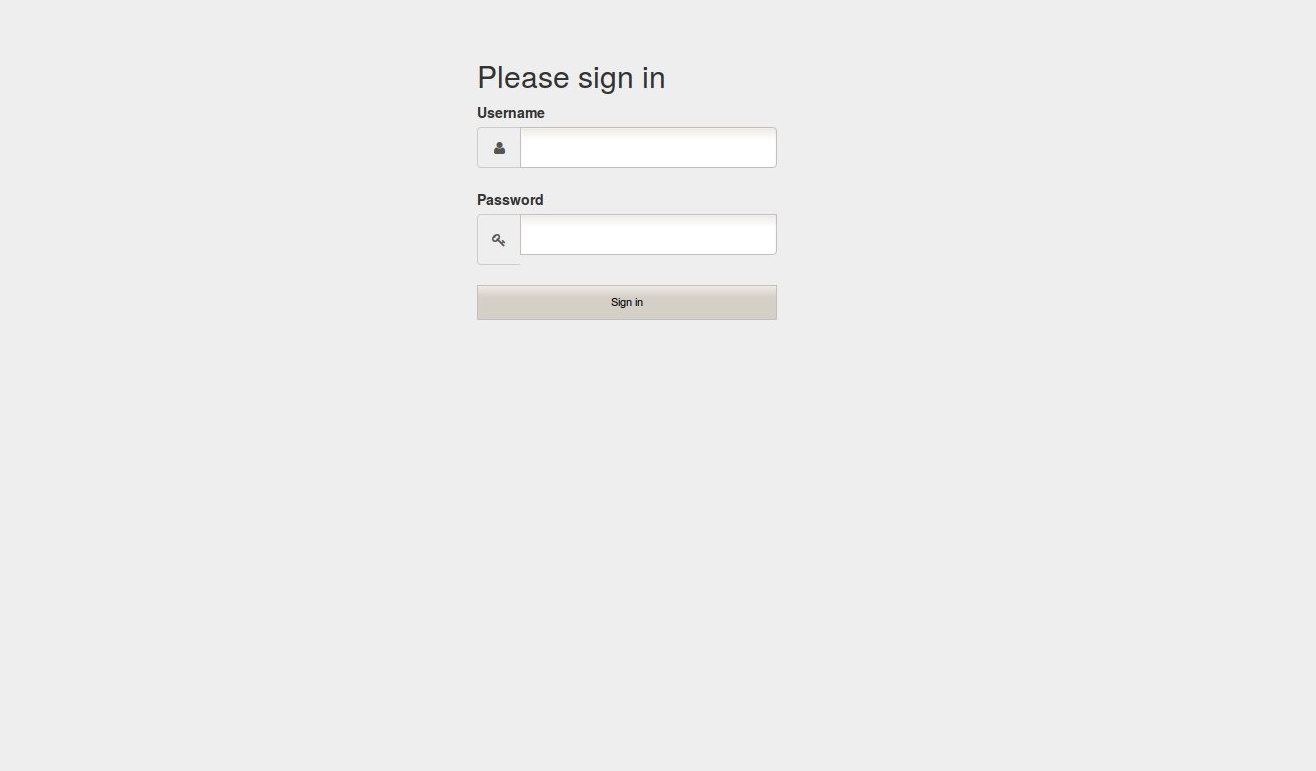
\includegraphics[scale=0.4]{login.jpg} 
\caption{Prihlasovacia obrazovka}



\end{center}

\end{figure}

	\begin{figure}[htb]

\begin{center}

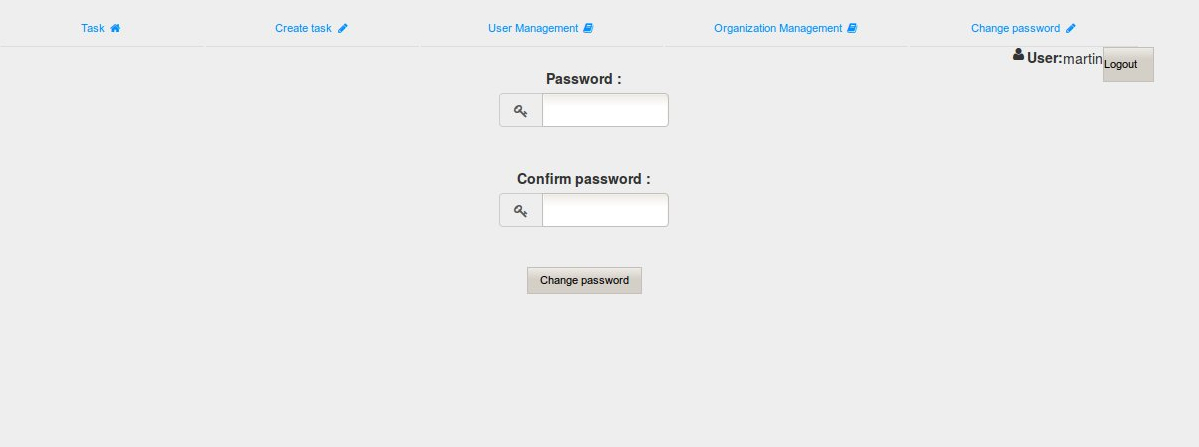
\includegraphics[scale=0.4]{page5.jpg} 
\caption{Zmena hesla}



\end{center}

\end{figure}



\begin{figure}[htb]

\begin{center}

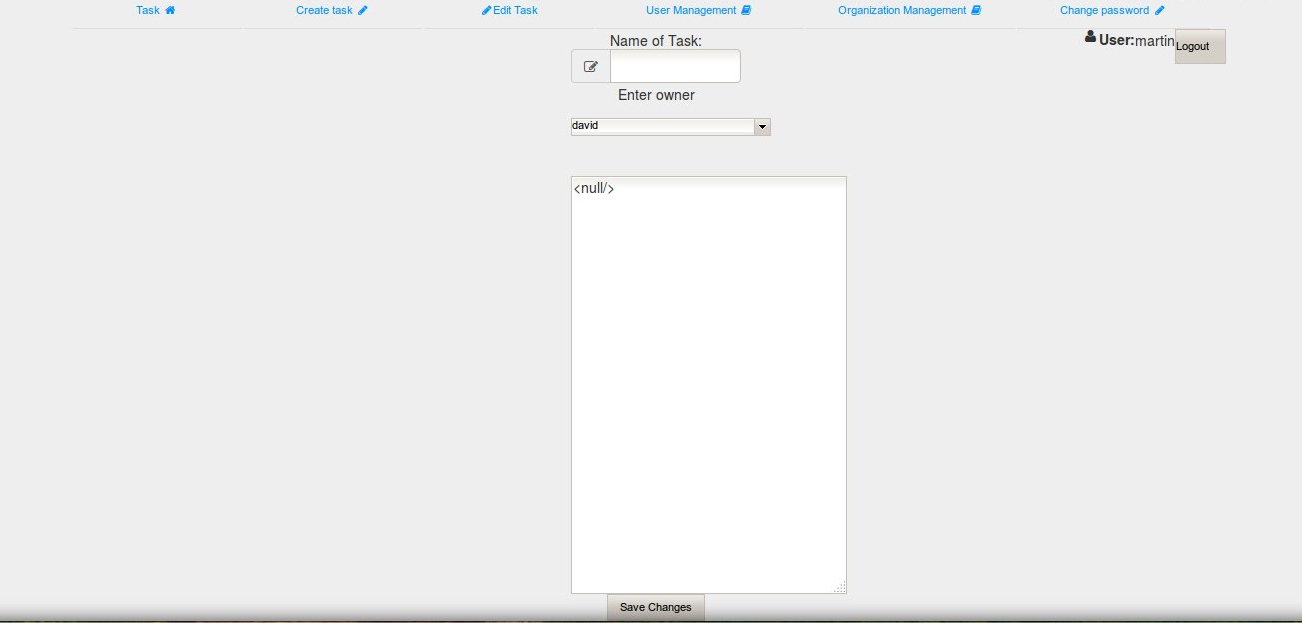
\includegraphics[scale=0.4]{page1.jpg} 
\caption{Editovanie úlohy}


\end{center}

\end{figure}

\begin{figure}[htb]

\begin{center}

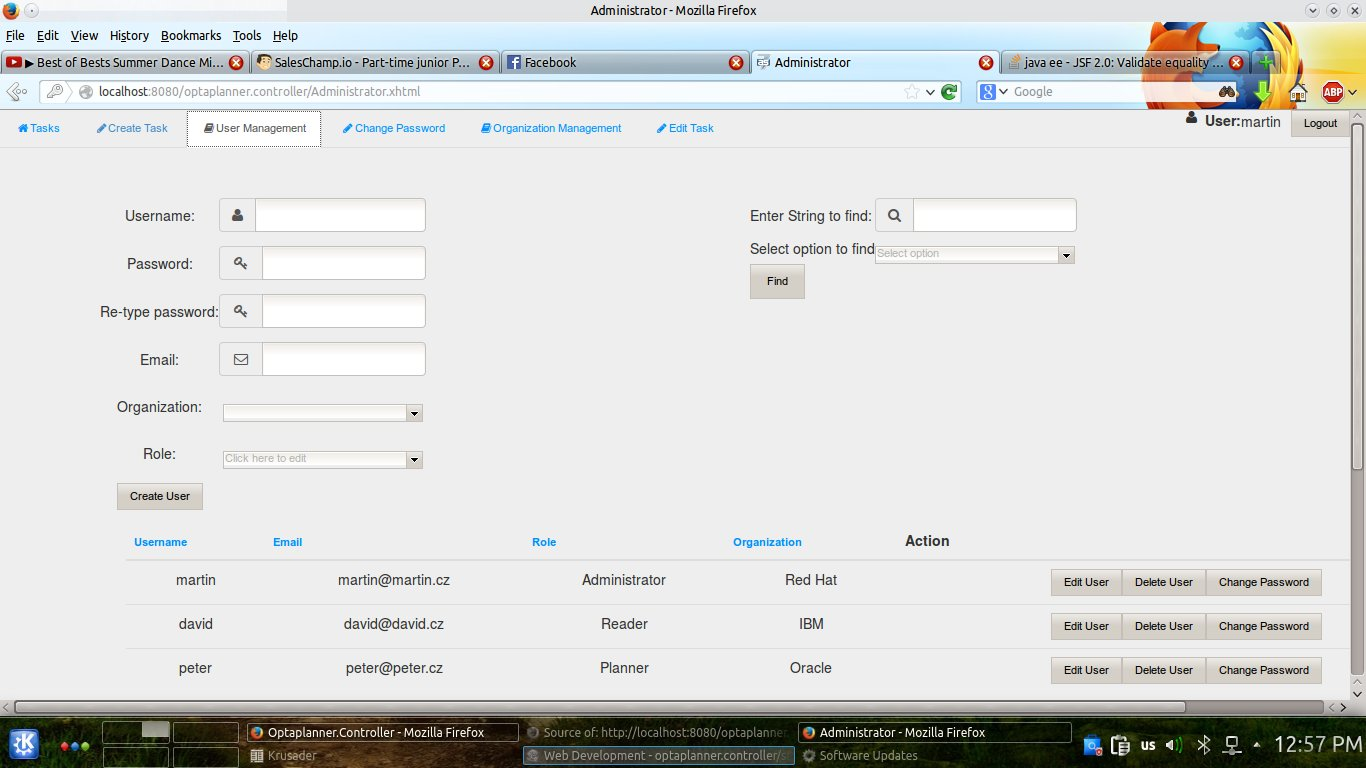
\includegraphics[scale=0.4]{page2.jpg} 
\caption{Nahrávanie novej úlohy}



\end{center}

\end{figure}


\begin{figure}[htb]

\begin{center}

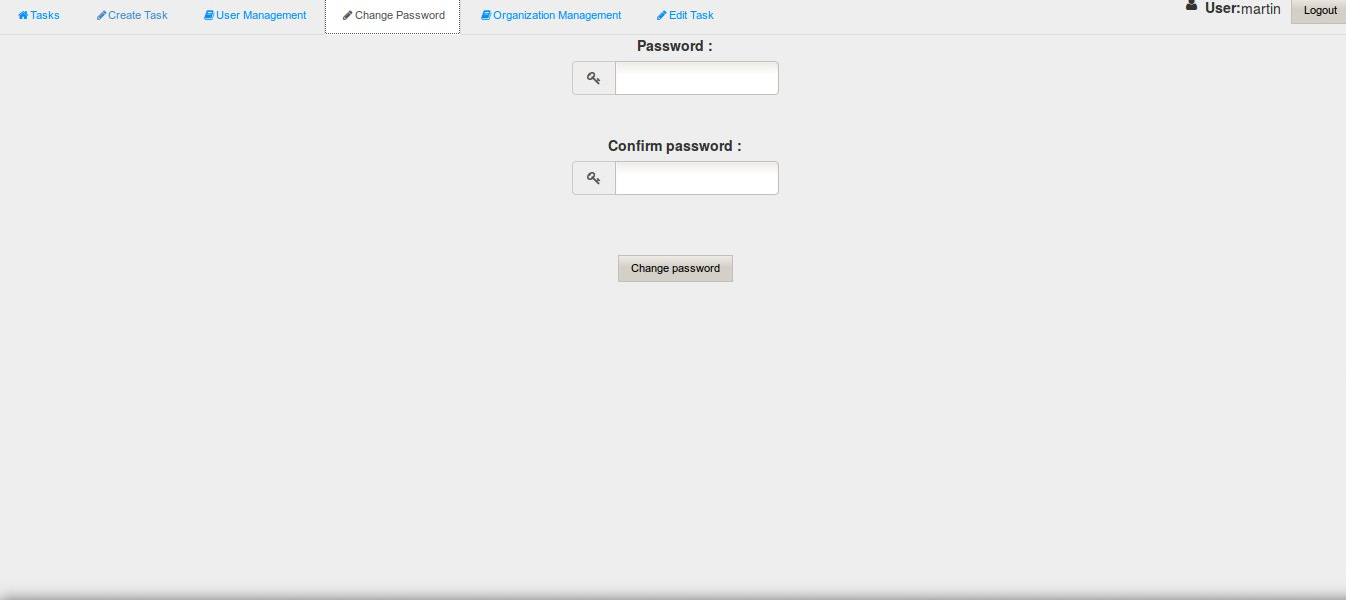
\includegraphics[scale=0.4]{page3.jpg} 
\caption{Spravovanie užívateľov}


\end{center}

\end{figure}

\begin{figure}[htb]

\begin{center}

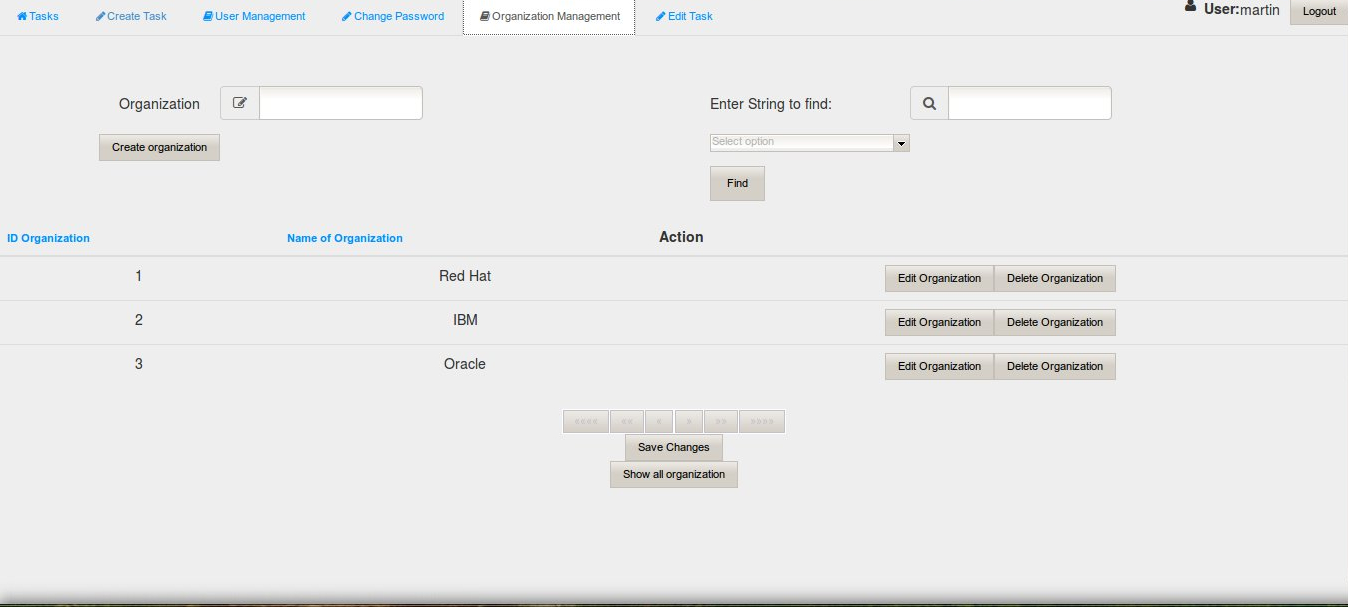
\includegraphics[scale=0.4]{page4.jpg} 
\caption{Spravovanie organizácií}


\end{center}

\end{figure}






}

\chapter{Dotazník}
{
	\section{Obsah dotazníka}
	{
\begin{figure}[htb]

\begin{center}

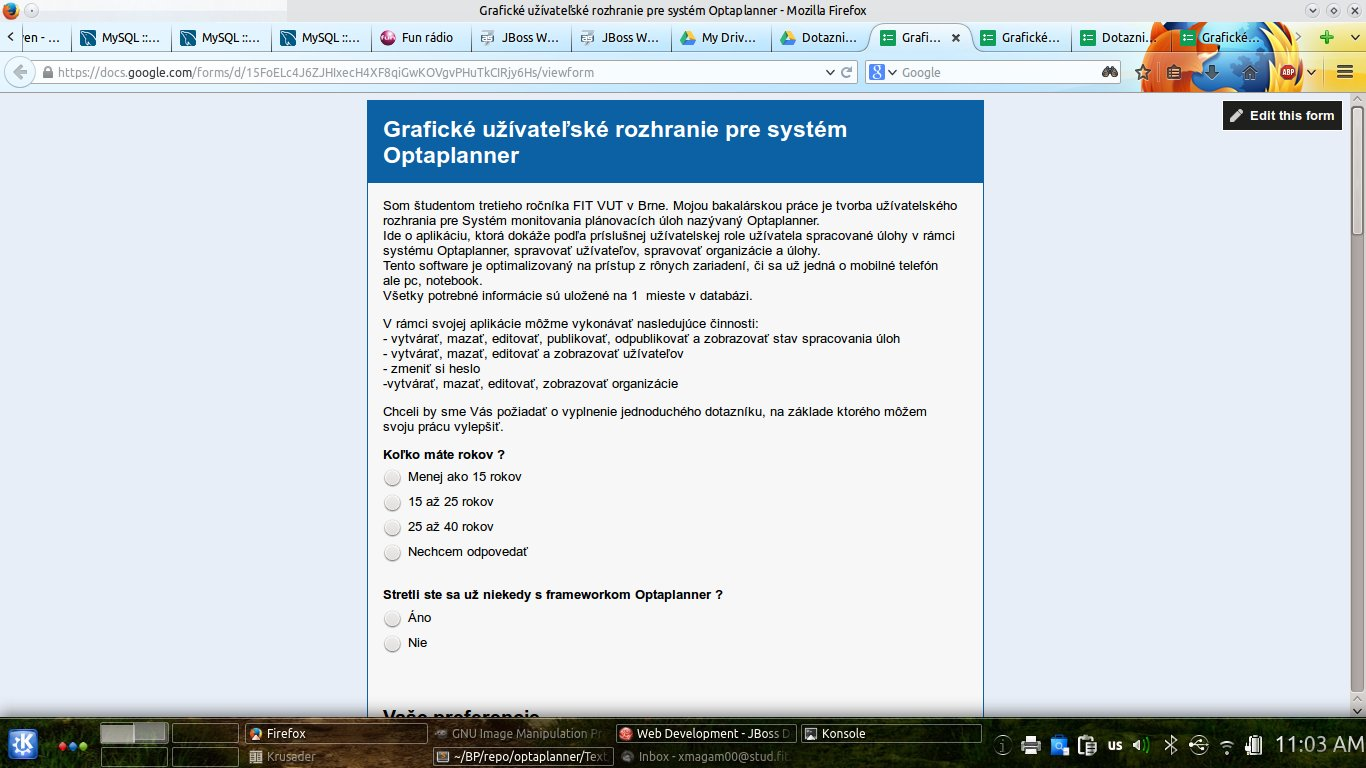
\includegraphics[scale=0.5]{dotaz.jpg} 
\caption{Všeobecné informácie}


\end{center}

\end{figure}


\begin{figure}[htb]

\begin{center}

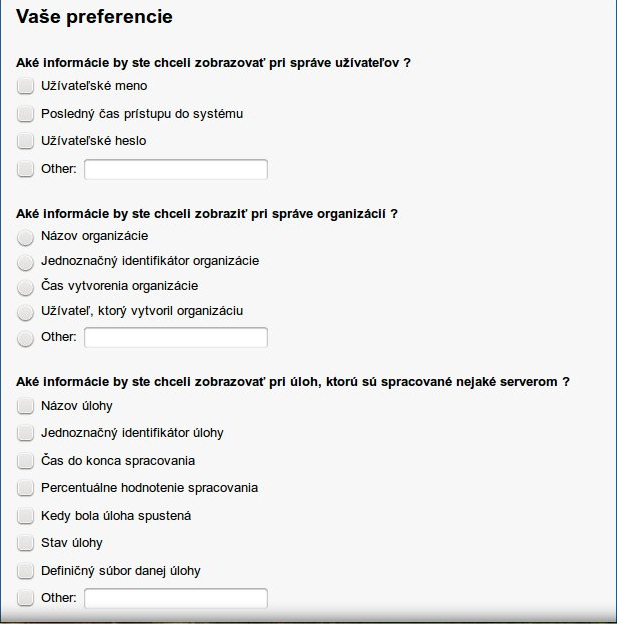
\includegraphics[scale=0.5]{dotaz1.jpg} 
\caption{Preferencie}


\end{center}

\end{figure}


\begin{figure}[htb]

\begin{center}

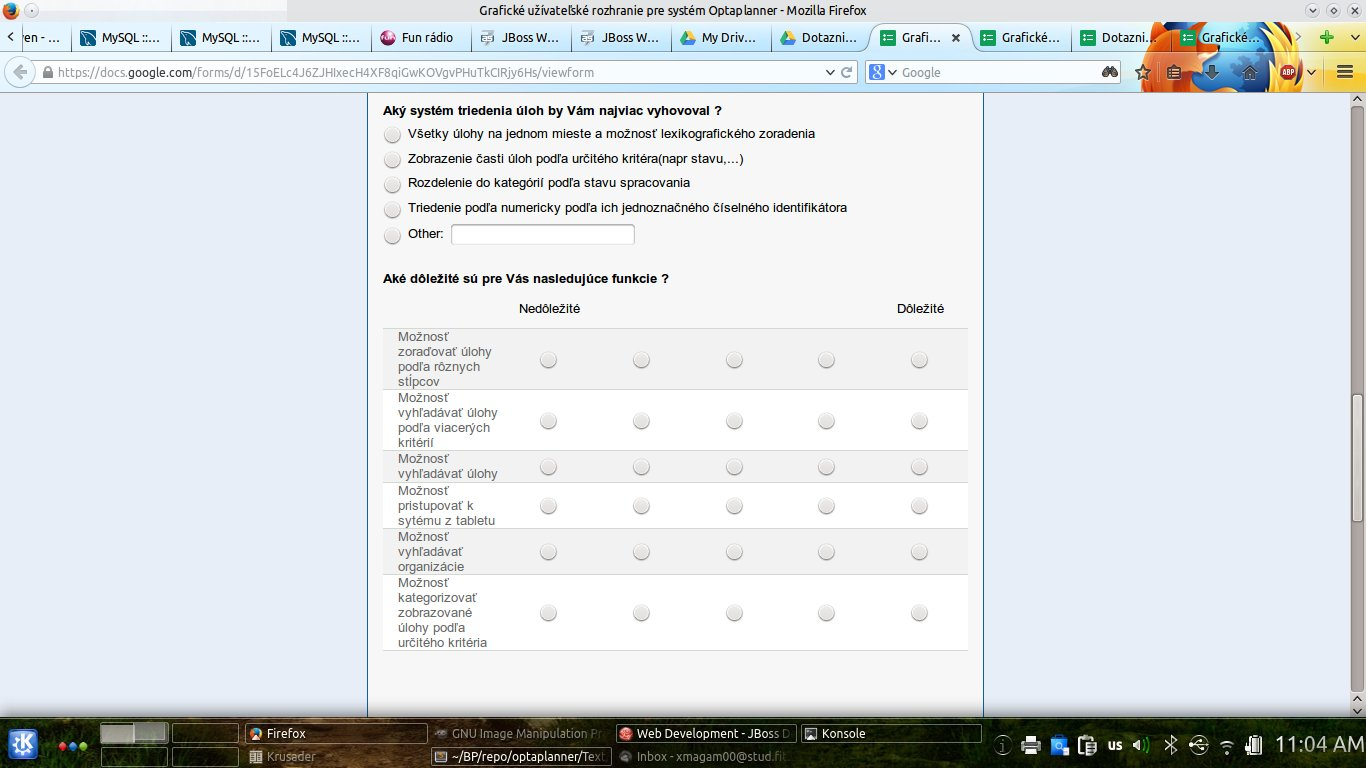
\includegraphics[scale=0.5]{dotaz2.jpg} 
\caption{Hodnotenie}


\end{center}

\end{figure}

\begin{figure}[htb]

\begin{center}

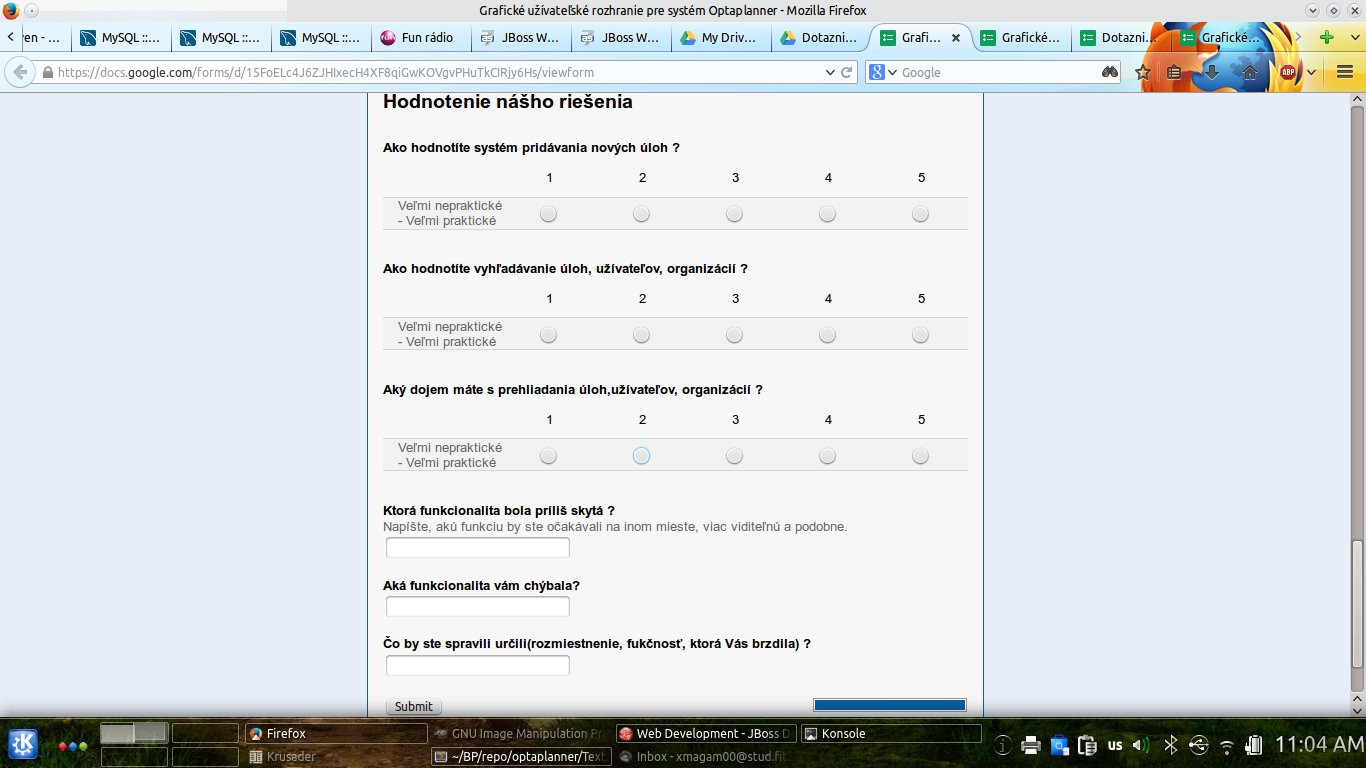
\includegraphics[scale=0.5]{dotaz3.jpg} 
\caption{Záverečné hodnotenie}


\end{center}

\end{figure}

	}


	


}

\chapter{CD so zdrojovými kódmi}
{
	Priložené CD obsahuje nasledujúce súbory:
	\begin{itemize}
	\item optaplanner.controller.war - adresár aplikácie pre užívateľské rozhranie obsahujúce preložené súbory vrátane potrebných súborov
	\item PlannerService.war - súbor s EJB a web service, ktorý obsahuje zdrojové kódy vrátane konfiguračných súborov
	\item install.txt - súbor s popisom inštalácie
	\item create.sql - sql súbor s definíciami tabuliek
	\item insert.sql sql súbor s naplnením dát tabuliek
	\item bachelor\_thesis.pdf - elektronická verzia textovej Časti bakálarskej práce
	\item mysql-connector-java-5.1.29-bin.jar - ovládač pre prácu s MySQL databázou
	\item 4queens.xml,8queens.xml, 16queens.xml - definičné súbory pre plánovací problém 4, 8 a 16 dám
	\item src - adresár, ktorý obsahuje zdrojové kódy k aplikácií pre užívateľské rozhranie(optaplanner.controller) a PlannerService
	\end{itemize}
}
%\chapter{RelaxNG Schéma konfiguraèního soboru}
%\chapter{Plakat}
